In origine era permessa l'esecuzione di un solo programma per macchina, il quale aveva il controllo totale della suddetta.

Ma oggi possiamo avviare potenzialmente centinaia di programmi contemporaneamente ed essi possono operare con un certo grado di indipendenza.

Ciò è possibile grazie al concetto di \textit{processo}, ossia ciò che in prima istanza definiamo come un programma in esecuzione, o, l'unità di lavoro dell'elaboratore.

Con la crescente complessità dei sistemi, cresce anche la necessità di gestione dei processi. Infatti, oltre ai programmi utente c'è anche necessità di gestire processi di sistema.

Un sistema è dunque composto da un insieme di processi: quelli del sistema operativo che eseguono il codice di sistema, e quelli utente che eseguono il codice utente.

\section{Concetto di Processo}
    La necessità di dare un nome al lavoro eseguito dalla CPU c'è sempre stato, e sono stati usati termini come \textit{task}, \textit{job}, eccetera. Anche un sistema monoutente esegue spesso multipli programmi, e anche nel caso dell'esecuzione di un singolo programma, ha bisogno di gestire una serie di attività interne. Queste unità di lavoro prendono comunemente il nome di \textbf{processi}.
    
    C'è da ricordare che in alcuni casi potrebbe essere usato il termine ormai superato \textit{job}, nel caso di terminologie ben stabilite come \textit{job scheduling}.
    
    \subsection{Il Processo}
        Lo stato dell'attività corrente di un processo è rappresentato dal valore del contatore di programma. La sua struttura interna è divisa in sezioni come descritto in figura.
        
        \begin{figure}[h]
            \centering
            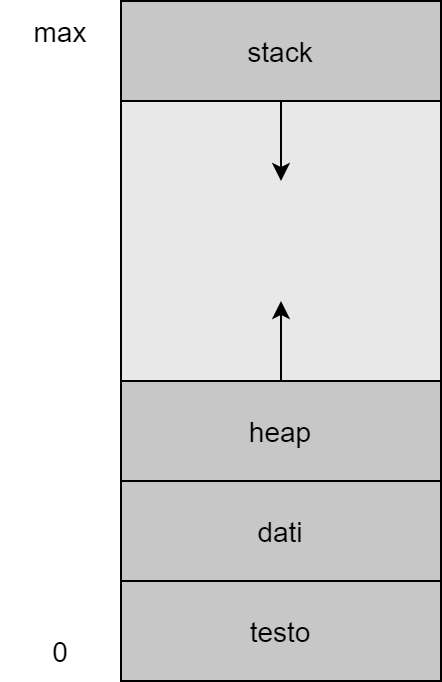
\includegraphics[width=0.3\textwidth]{img/img6.png}
            \caption{Struttura di un processo in memoria}
            \label{fig:img6}
        \end{figure}
        
        Le sezioni sono le seguenti:
        \begin{itemize}
            \item \textbf{Sezione di testo:} Contiene il codice eseguibile.
            \item \textbf{Sezione dati:} Contiene le variabili globali.
            \item \textbf{Heap:} Memoria allocata dinamicamente durante l'esecuzione del programma.
            \item \textbf{Stack:} Memoria temporaneamente utilizzata durante le chiamate di funzioni (parametri della funzione, indirizzi di ritorno, variabili locali).
        \end{itemize}
        
        È bene notare che le dimensioni di testo e dati sono fisse, in quanto vengono calcolate a tempo di compilazione, mentre quelle di heap e stack sono dinamiche, e possono variare durante l'esecuzione.
        
        Ogni volta che viene richiamata una funzione, un \textbf{record di attivazione} contenente i suoi parametri, le variabili locali e l'indirizzo di ritorno viene aggiunto allo stack; quando la funzione restituisce il ritorno al chiamante, il record viene rimosso dallo stack.
        
        Al contrario, lo heap cresce quando viene allocata memoria dinamicamente e diminuisce in dimensioni quando la memoria viene restituita al sistema. Lo stack e lo heap crescono \textit{l'uno verso l'altro}, quindi sta al sistema operativo assicurare che non si sovrappongano.
        
        \textbf{Un programma non è un processo.} Un programma è un'entità \textit{passiva}, come un file su disco contenente una lista di istruzioni, mentre un processo è un'entità \textit{attiva}, con un contatore di programma che indica l'istruzione successiva da eseguire e un insieme di risorse associate. Un programma diventa processo quando il file eseguibile viene caricato in memoria.
        
        Sebbene \textbf{due o più processi} possano essere associati allo stesso programma, vanno considerati come due entità diverse, in quanto le altre risorse (dati, heap e stack) sono diverse.
        
    \subsection{Stato del processo}
        Un processo ha uno \textbf{stato}, e questo è soggetto a cambiamenti durante la sua esecuzione. Ecco i possibili stati di un processo:
        \begin{itemize}
            \item \textbf{Nuovo.} Si crea il processo.
            \item \textbf{Esecuzione (\textit{running}).} Le sue istruzioni vengono eseguite.
            \item \textbf{Attesa (\textit{waiting}).} Il processo aspetta che si verifichi un evento, come un'operazione I/O o la ricezione di un segnale.
            \item \textbf{Pronto (\textit{ready}).} Il processo attende di essere assegnato a un'unità di elaborazione.
            \item \textbf{Terminato.} Il processo ha terminato l'esecuzione.
        \end{itemize}
        
        Questi termini sono abbastanza arbitrati, ma i concetti che rappresentano sono presenti in tutti i sistemi operativi, nonostante alcuni sistemi aggiungano ulteriori distinzioni fra gli stati.
        
        È bene tenere a mente che su un'unità di elaborazione un solo processo può essere \textit{running}, anche se molti possono essere in stato di \textit{waiting} o \textit{ready}. In basso è riportato il diagramma di transizione fra gli stati.
        
        \begin{figure}[h]
            \centering
            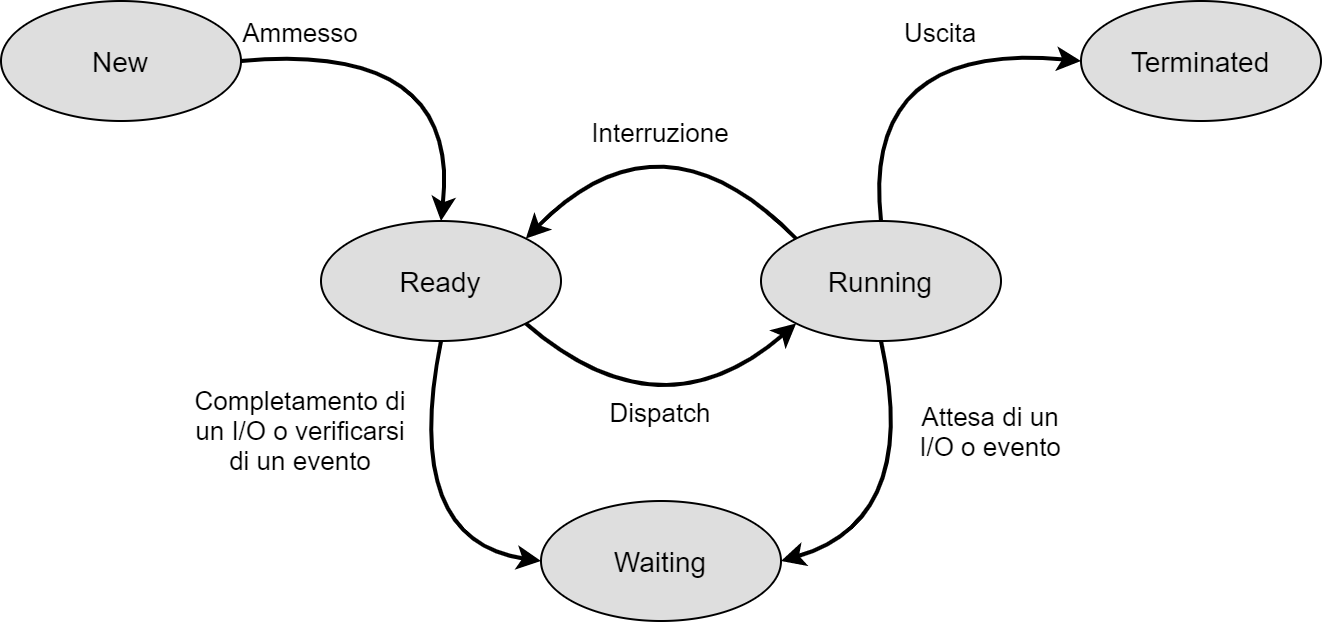
\includegraphics[width=0.9\textwidth]{img/img7.png}
            \caption{Diagramma di transizione degli stati di un processo.}
            \label{fig:img7}
        \end{figure}
        
    \subsection{Blocco di controllo del processo}
        Ogni processo è rappresentato nel sistema operativo da un \textbf{PCB}, \textit{process control block}, il quale contiene molte informazioni connesse a un processo, fra cui le seguenti:
        \begin{itemize}
            \item \textbf{Stato del processo.}
            \item \textbf{Contatore di programma.} Contiene l'indirizzo della seguente istruzione da eseguire per tale processo.
            \item \textbf{Registri della CPU.} Essi variano in numero e tipo in base all'architettura del calcolatore, ma possono includere accumulatori, registri indice, etc.
            \item \textbf{Informazioni sullo scheduling di CPU.}
            \item \textbf{Informazioni sulla gestione della memoria.} Possono includere diverse informazioni in base al sistema di gestione della memoria usato dal sistema operativo, fra cui valore dei registri di base e di limite, tabelle delle pagine o dei segmenti, etc.
            \item \textbf{Informazioni di accounting.} Includono la quota e il tempo di uso della CPU, i limiti di tempo, i numeri dei processi, etc.
            \item \textbf{Informazioni sullo stato dell'I/O.} Lista dei dispositivi assegnati a un dato processo, lista dei file aperti, etc.
        \end{itemize}
        
        In sintesi, il PCB si usa semplicemente come deposito per tutte le informazioni relative ai vari processi.
        
    \subsection{Thread}
        Fino ad ora abbiamo dato per scontato che un processo segue un singolo percorso di esecuzione, una singola sequenza di istruzioni, pur riservandosi il privilegio di metterla in pausa per avviarne temporaneamente un'altra.
        
        Questo paradigma è tuttavia limitante, specialmente nei sistemi multicore, ed infatti viene introdotto il concetto di \textbf{thread}, ossia un percorso di esecuzione che può essere eseguito in parallelo con altri. Le relative informazioni necessarie ai thread vengono aggiunte al PCB.
        
\section{Scheduling dei processi}
    L'obiettivo della multiprogrammazione è quello di tenere sempre almeno un processo attivo, e idealmente tanti quanti ne sono le CPU. Quando un processo va in stato di attesa, lo \textbf{scheduler dei processi} va a selezionarne un altro dalla lista dei processi in attesa. Lo scopo è ovviamente quello di massimizzare l'utilizzo della CPU. Il numero di processi in memoria in un dato istante è detto \textbf{grado di multiprogrammazione}.
    
    È bene considerare inoltre anche la natura dei processi. Parliamo di processi \textbf{I/O bound} nel caso di processi che impiegano la maggior parte del loro tempo in operazioni di lettura e scrittura, mentre parliamo di processi \textbf{CPU bound} nel caso di processi che impiegano la maggior parte del loro tempo in operazioni di elaborazione.
    
    \subsection{Code di scheduling}
        Ogni processo è inserito in una coda di processi pronti chiamata \textit{ready queue}, e sono generalmente implementati come liste concatenate.
        
        Supponiamo che un processo venga assegnato a un core della CPU, ma che in un certo momento esso richieda un input da parte di un disco o tastiera, operazioni generalmente molto lente. Esso, mentre è in attesa di tale input, viene posizionato in una coda d'attesa chiamata \textit{wait queue}.
        
        Un \textbf{nuovo processo} viene inizialmente posizionato nella ready queue fino a che non viene selezionato per essere eseguito (\textit{dispatched}). A questo punto inizia a eseguire le sue elaborazioni e si può verificare uno dei seguenti scenari:
        \begin{itemize}
            \item Il processo può emettere una richiesta di I/O e quindi essere assegnato a una coda di I/O.
            \item Il processo può creare un nuovo processo figlio e attenderne la terminazione.
            \item Il processo può essere rimosso forzatamente dalla CPU a causa di una interruzione ed essere messo nella coda dei processi pronti.
        \end{itemize}
        
        Un processo continua questo ciclo fino al completamento della sua esecuzione: a questo punto viene rimosso da tutte le code e vengono deallocati il suo PCB e le sue risorse.
        
        \begin{figure}[h]
            \centering
            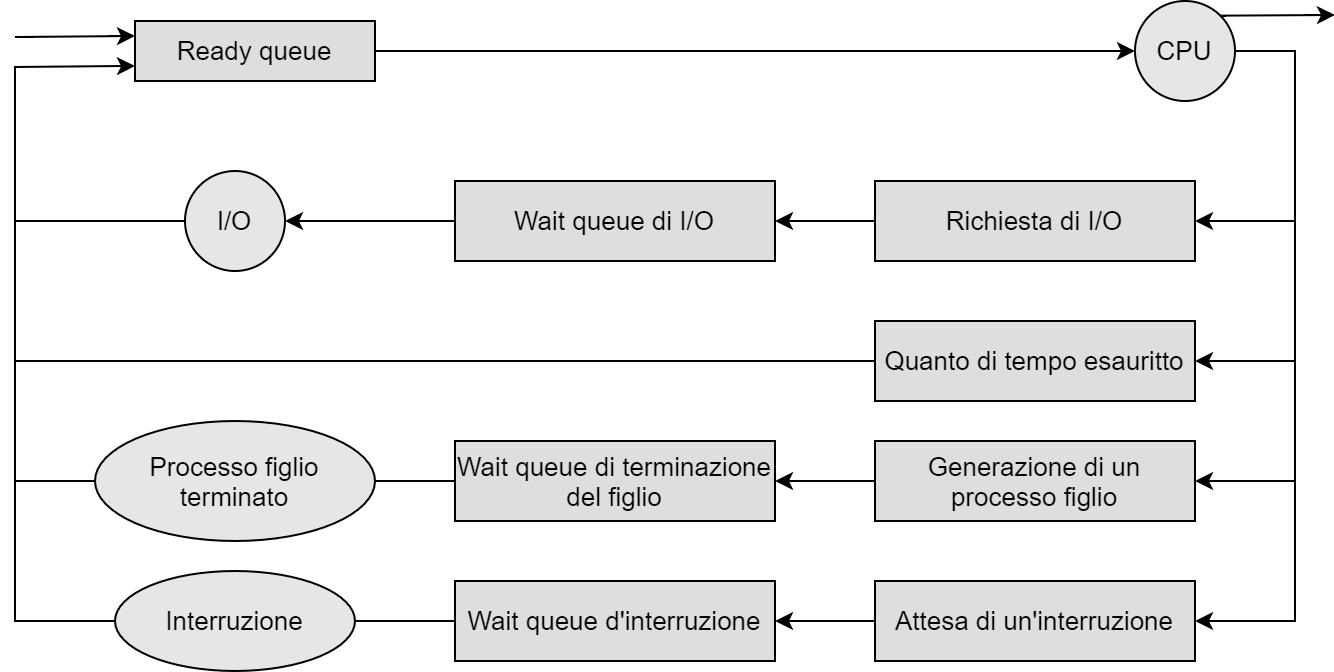
\includegraphics[width=0.95\textwidth]{img/img8.png}
            \caption{Diagramma di accodamento per lo scheduling dei processi.}
            \label{fig:img8}
        \end{figure}
        
    \subsection{Scheduling della CPU}
        Un processo pronto deve essere assegnato a un core della CPU per consentirne l'esecuzione, ed è proprio questo il compito dello scheduler della CPU.
        
        Un processo \textbf{I/O bound} potrà restare in esecuzione per pochi millisecondi prima di tornare in attesa di un input, mentre un processo \textbf{CPU bound} potrà restare in esecuzione per un tempo più lungo. Tuttavia è improbabile che lo scheduler della CPU lasci in esecuzione processi per periodi prolungati. Tenderà invece a rimuovere forzatamente un processo dalla CPU per metterlo in attesa, così da non dare la possibilità a nessun processo di monopolizzare le risorse.
        
        Alcuni sistemi operativi hanno una forma intermedia di scheduling, chiamata \textbf{swapping}. Questa tecnica prevede la rimozione di un processo dalla memoria (\textit{swap-out}) per diminuire il grado di multiprogrammazione e quindi la contesa per la CPU, per poi reintrodurre il processo swappato (\textit{swap-in}) in seguito, nello stato in cui è stato lasciato l'ultima volta. Questo schema è solitamente utilizzato solo quando abbiamo un sovraccarico di memoria.
        
    \subsection{Cambio di contesto}
        Quando un'interruzione forza il sistema a sospendere il lavoro attuale della CPU, c'è necessità di salvare il \textbf{contesto} del processo corrente, per poterlo ripristinare in seguito.
        
        Il contesto è rappresentato all'interno del PCB del processo, e comprende i valori dei registri della CPU, lo stato del processo e informazioni relative alla gestione della memoria. In termini generali parliamo di \textbf{salvataggio dello stato} corrente della CPU e susseguentemente \textbf{ripristino dello stato}.
        
        Il passaggio della CPU a un nuovo processo implica il salvataggio del contesto corrente e il ripristino del contesto del nuovo processo. Questa procedura è chiamata \textbf{cambio di contesto}, o \textit{context switch}. Il context switch è puro overhead, siccome il sistema esegue operazioni atte alla gestione dei processi senza nessun tipo di computazione.

\section{Operazioni sui processi}
    Il sistema operativo deve fornire metodi per creare e cancellare i processi, i quali devono poter essere cariati e rimossi dinamicamente.
    
    \subsection{Creazione di processi}
        Un processo può creare altri processi. Il processo che crea viene chiamato processo \textbf{genitore}, o \textbf{padre}, mentre il processo creato viene chiamato processo \textbf{figlio}. Questo processi possono creare altri processi, creando così un \textbf{albero} di processi.
        
        La maggior parte dei sistemi operativi identifica un processo per mezzo di un numero unico, solitamente un intero, chiamato \textbf{identificatore del processo} o \textbf{pid} (\textit{process identifier}). Questo è utile per identificare univocamente i processi e gestirli.
        
        In Linux (dove generalmente si preferisce il termine \textit{task} ma qui usiamo processo in maniera generica), abbiamo per esempio \texttt{systemd} che è il processo padre di tutti i processi utente e ha sempre \texttt{pid} uguale a 1.
        
        Solitamente un processo figlio avrà bisogno di determinante risorse, fra cui dispositivi di I/O, memoria, etc. Può ottenere queste risorse direttamente dal sistema operativo oppure ereditarle dal processo padre. Quando un processo va a creare figli può spartire le proprie risorse o una sottoinsieme di esse fra i figli. Questa cosa ha fra l'altro lo scopo di non sovraccaricare troppo il sistema, cosa che potrebbe succedere se un processo iniziasse a creare figli affamati di risorse in maniera incontrollata. Oltre a risorse il processo padre può passare ai figli anche dei parametri di inizializzazione.
        
        Quando un processo ne crea uno nuovo, ci sono due possibilità per quanto riguarda l'esecuzione:
        \begin{enumerate}
            \item Il processo genitore continua la sua esecuzione in maniera concorrente con i propri figli.
            \item Il processo genitore attente che alcuni o tutti i suoi figli terminino.
        \end{enumerate}
        
        Ci sono allo stesso modo due possibilità per quanto riguarda lo spazio di indirizzi del nuovo processo:
        \begin{enumerate}
            \item Il processo figlio è un duplicato del processo genitore (ha stessi programma e dati).
            \item Nel processo figlio si carica un nuovo programma.
        \end{enumerate}
        
    \subsection{Terminazione di un processo}
        Un processo termina quando finisce l'esecuzione della sua ultima istruzione e inoltra la richiesta al sistema operativo di essere cancellato. Il processo può riportare un'informazione di stato al processo padre, e tutte le risorse occupate, comprese memoria fisica e virtuale, file e dispositivi di I/O vengono liberati dal sistema operativo.
        
        Un processo può anche terminare prematuramente, e questa operazione è eseguita dal genitore. Il motivo è di sicurezza, in quanto se così non fosse un utente potrebbe arbitrariamente provocare la terminazione di qualsiasi processo. Un genitore deve, quindi, conoscere le identità dei propri figli per terminarli, ed è per questo che quando un processo viene creato, la propria identità viene passata al processo genitore.
        
        Un processo genitore può porre termine all'esecuzione di uno dei suoi processi figli per vari motivi, fra quali i seguenti:
        \begin{itemize}
            \item Il processo figlio ha ecceduto nell'utilizzo di alcune risorse che gli sono state concessi. Ciò richiede che il processo padre disponga di informazioni circa lo stato dei propri figli.
            \item Il compito assegnato al processo figlio non è più richiesto.
            \item Il processo genitore termina e il sistema operativo non consente l'esistenza di tali situazioni.
        \end{itemize}
        
        In alcuni sistemi operativi, se un processo termina, terminano anche tutti i suoi figli, a prescindere dalla natura della terminazione (normale o anormale). In questo caso si parla di \textbf{terminazione a cascata}.
        
        Quando un processo termina le sue risorse vengono deallocate dal sistema operativo. Tuttavia, la sua voce nella tabella dei processi deve rimanere fino a quando il padre chiama \texttt{wait()}, perché la tabella dei processi contiene lo stato di uscita del processo.
        
        Un processo che è terminato, ma il cui genitore non ha ancora chiamato la \texttt{wait()}, è detto processo \textbf{zombie}. Tutti i processi entrano in questo stato dopo la loro terminazione, ma solitamente ci restano solo per breve tempo. Una volta che il loro genitore chiama la \texttt{wait()}, il \textit{pid} del processo zombie e la sua voce nella tabella dei processi vengono rilasciati.
        
        Consideriamo ora un genitore che termina senza invocare la \texttt{wait()}. Esso lascia i processi figli come orfani. Alcuni sistemi operativi, come Linux e UNIX, affrontano questa situazione facendo diventare il processo radice (\texttt{init} per UNIX e \texttt{systemd} per Linux) il nuovo genitore dei processi orfani. Inoltre il processo radice chiama periodicamente la \texttt{wait()} per liberare le risorse.
        
    \subsection{Comunicazione tra processi}
        Processi eseguiti concorrentemente nel sistema operativo possono essere \textit{indipendenti}, nel caso in cui non influiscano o subiscano l'influenza di altri processi durante la loro esecuzione, o \textit{cooperanti} nel caso contrario. Ovviamente l'essere o meno indipendente è fortemente collegato alla condivisione di dati fra processi.
        
        Alcuni motivi dell'utilità di un ambiente che consente la cooperazione fra processi:
        \begin{itemize}
            \item \textbf{Condivisione d'informazioni:} In questo modo più utenti possono accedere concorrentemente a risorse a cui sono interessate, come un file condiviso.
            
            \item \textbf{Velocizzazione del calcolo:} Se l'elaboratore dispone di più core di elaborazione, alcune attività possono essere suddivide in sottoattività eseguibili in parallelo, causando un aumento delle prestazioni.
            
            \item \textbf{Modularità:} Può essere utile la costruzione di un sistema modulare, che consente la suddivisione di funzioni di sistema in processi o thread.
        \end{itemize}
        
        Necessitiamo quindi di un meccanismo di comunicazione fra processi (\textbf{IPC}, \textit{interprocess comunication}). I due modelli principali sono quello a \textbf{memoria condivisa}, in cui si stabilisce una zona di memoria condivisa dai processi cooperanti, che possono leggere e scrivere da tale zona, e quello a \textbf{scambio di messaggi}.
        
        Io modello a memoria condivisa è più rapido, ma potrebbe creare problemi di sincronizzazione e accesso concorrente, mentre quello a scambio di messaggi è più facile da implementare, meno prono agli errori ma anche meno efficiente, e infatti è usato per scambiare piccole moli di dati. Nei sistemi operativi moderni troviamo entrambi i modelli, spesso nello stesso sistema.